\documentclass{book}
\usepackage{M.1.0.0}
\newcommand{\specialcell}[2][c]{%
  \begin{tabular}[#1]{@{}c@{}}#2\end{tabular}}

%  % % % % % % % % % % % % % % % % % % % % % % % % % % % % % % % % % % % %
%
%                                                                 INICIO DEL DOCUMENTO 
% % % % % % % % % % % % % % % % % % % % % % % % % % % % % % % % % % % % %

%  % % % % % % % % % % % % % % % % % % % % % % % % % % % % % % % % % % % %
\begin{document}

\Ini


\chapter*{Prefacio}

Contenido del prefacio. 

\tableofcontents 

\Figura

\Cuadros


\Res{T\'itulo del resumen}
                  
Aqu\'i va el texto del resumen

\Chapter{Introducci\'on}
\UnoA

El presente Megaproyecto tiene como objetivo dise\~nar y construir un detector de radiaci\'on Cherenkov de agua (WCD por sus siglas en ingl\'es) para tomar y procesar datos en la determinaci\'on de eventos atmosf\'ericos como consecuencia de reducci\'on Forbush. Al culminar la realizaci\'on de este proyecto se pretende promover un intercambio generacional de conocimientos de part\'iculas de altas energ\'ias, contribuir el \'area de investigaci\'on de este tipo en Guatemala, colaborar con la recopilaci\'on de informaci\'on por parte de observatorios LAGO, y servir como referencia para la construcci\'on de observatorios similares a mayores altitudes en otras regiones del pa\'is.

El m\'odulo de f\'isica en este megaproyecto abarca la caracterizaci\'on de se\~nal de eventos. Esto incluye la elaboraci\'on de una simulaci\'on Monte Carlo de eventos en el tanque y la elaboraci\'on de estrategias para la calibraci\'on de datos y la identificaci\'on de part\'iculas a partir de la se\~nal de eventos. La simulaci\'on Monte Carlo tiene como objetivo caracterizar el conteo de fotones por el fotomultiplicador para el evento de un mu\'on o gamma secundario, y se realizar\'a utilizando la herramienta GEANT4 desarrollada por CERN. El resultado de esta simulaci\'on ser\'a una completa descripci\'on de la forma esperada de la se\~nal en el fotomultiplicador para un evento t\'ipico de mu\'on que atravieza el tanque, mu\'on que decae y el electr\'on que produce, y rayos gamma que producen pares, y esto para diferentes \'angulos de incidencia y a lo largo del espectro de energ\'etico de un mu\'on o rayo gamma como part\'icula secundaria proveniente de una cascada extensa. Esta descripci\'on es crucial para cumplir con el objetivo perteniente a la determinaci\'on de la identidad de las part\'iculas que generan los eventos que observaremos ya que la forma de la se\~nal que obtendremos del multiplicador ser\'an comparadas con los resultados de la simulaci\'on con fines de calibraci\'on.


\Chapter{Objetivos}

\section{Objetivo general}
Calibrar las se\~nales obtenidas del fototubo dentro del WCD utilizando el modo de histograma y comparando con simulaci\'on Monte Carlo con Geant4.
\section{Objetivos espec\'ificos}
\begin{itemize}
 \item Obtener la calibraci\'on por el mu\'on vertical equivalente (VEM) a partir de la simulaci\'on y compararlo con el an\'alisis de primer nivel de los datos de ACQUA del montaje experimental del tanque.
 \item Calcular la vida media del mu\'on a partir de una corrida del experimento en el WCD.
 \item Obtener la forma representativa de pulsos en el tiempo con la simulaci\'on en geant4 para muones que atraviesan, muones que decaen, electrones, sus antipartículas respectivas, y partículas gamma.
\end{itemize}

%%%%%%%%%%%%%%%%Cap\'itulo nuevo

\Chapter{Justificaci\'on}

Ya que la actividad solar y eventos en el medio interplanetario tienen efectos disruptivos sobre la magnet\'osfera, el estudio del efecto de fen\'omenos solares desde diferentes posiciones en la Tierra es muy valioso para prevenir da\~nos sobre sat\'elites y problemas en transmisiones de radio.

Por otro lado, este es uno de los pocos proyectos de f\'isica experimental en Guatemala, por lo que su valor formativo en el trabajo cient\'ifico en nuestra comunidad es importante ya que establecer\'a una plataforma para continuar la investigaci\'on de part\'iculas de altas energ\'ias de origen astrof\'isico. El intercambio generacional que originar\'a el proyecto, as\'i como su mantenimiento y replicaci\'on ser\'an formativos para estudiantes de f\'isica, qu\'imica e ingenier\'ias. Adem\'as, el trabajo en la electr\'onica de instrumentaci\'on del proyecto ser\'a un gran avance en el desarrollo tecnol\'ogico del pa\'is.

%%%%%%%%%%%%%%%%Cap\'itulo nuevo

\Chapter{Marco Te\'orico}

\section{Rayos c\'osmicos}
\subsection{Generalidades y descubrimiento de los rayos c\'osmicos}
Los rayos c\'osmicos son part\'iculas, con excepci\'on de fotones, que se originan fuera del Sistema Solar y llegan a la Tierra o su entorno cercano. Generalmente estas part\'iculas son n\'ucleos at\'omicos, desde hidr\'ogeno hasta de hierro. En la literatura, se les denomina tambi\'en <<primarios>>, especialmente en el contexto de cascadas de \'area extensa (descritas en la siguiente secci\'on. Los rayos c\'osmicos fueron descubiertos porque en laboratorios de f\'isica se observava que electr\'ometros cargados y aislados de fuentes radioactivas se descargaban sin aparente raz\'on. \citep{ASOREY}

Theodor Wulf a los inicios del siglo XX desarroll\'o un electroscopio m\'as sensible y not\'o que en la punta de la Torre Eiffel la tasa de decaimiento era mayor de la esperado tomando \'unicamente la radiaci\'on gamma, como pensado en esa \'epoca. Por otro lado, Domenico Pacini, realiz\'o tres mediciones: a nivel del suelo, en la superficie del Lago Bracciano, y a tres metros de profundidad en el lago. Comparando estas mediciones, en las que se destacaba que bajo el agua la tasa disminu\'ia, concluy\'o que debe de haber una fuente de radiaci\'on adicional. \citep{ASOREY}

V.F. Hess en 1912 fue quien finalmente dijo que la fuente de esta radiaci\'on es de origen extraterrestre y que ingresa desde arriba de la atm\'osfera con gran poder penetrante. El experimento que realiz\'o le gan\'o el Nobel de F\'isica en 1936. Consist\'ia en la medici\'on de tasas de ionizaci\'on a diferentes altitudes. Las mediciones las realiz\'o durante 10 vuelos en globos aereost\'aticos hasta los 5000 m.s.n.m. La dependencia de la tasa de ionizaci\'on sobre la altitud fue lo que llev\'o a su importante conclusi\'on. \citep{ASOREY}

Los rayos c\'osmicos tienen un rango de energ\'ia extremadamente amplio: desde $10^5 eV$, que incluye part\'iculas del viento solar hasta $10^20 eV$, part\'iculas intergal\'acticas. Los rayos c\'osmicos de ultra alta energ\'ia son primarios con energ\'ias superiores a $E_p \geq 10^18 eV$. Su medici\'on directa es casi imposible debido al baj\'isimo flujo. En cambio, se infiere su existencia por la detecci\'on de las part\'iculas secundarias producidos por la cascada de \'area extensa producida por el ingreso del primario. Esto fue observado por primera vez en 1934 por Bruno Rossi quien not\'o que equipos separados por gran distancia detectaban simult\'aneamente aumentos en el conteo de part\'iculas; Pierre Auger infiri\'o en 1938 que esto era explicado por el ingreso de una part\'icula primaria de energ\'ias superiores a los $10^15 eV$. \citep{ASOREY}

Los modelos de aceleraci\'on explican c\'omo estas part\'iculas pueden alcanzar energ\'ias tan altas. Un mecanismo de aceleraci\'on es cuando RC atraviesan una nube de gas en el medio interplanetario. El efecto de esta interacci\'on es un aumento en la energ\'ia del RC. Sin embargo, este aumento es ineficiente a menos que la velocidad propia de la nube sea de magnitudes relativistas ($\beta\approx1$), como con los frentes de choque producidos por supernovas. Sin embargo, estos modelos sufren a\'un de sobresimplificaci\'on, ya que consideran la densidad en los frentes de choque como funciones escal\'on y que el frente es no relativista, por lo que la explicaci\'on de rayos c\'osmicos de ultra alta energ\'ia es todav\'ia un problema abierto. \citep{ASOREY}

\subsection{Espectro de rayos c\'osmicos}

\section{Actividad solar y rayos c\'osmicos}

Estos fen\'omenos consisten en la variaci\'on r\'apida de la intensidad de los rayos c\'osmicos, seguida por una eyecci\'on coronal desde el Sol. Este efecto fue descubierto por Scott E. Forbush en 1937, que tambi\'en observ\'o que la intensidad de los RC al alcanzar la Tierra se encontraban inversamente correlacionados con los 11 a\~nos de ciclo solar de las manchas solares. Un detector que lleve la cuenta permanente de los rayos c\'osmicos que llegan a tierra puede dar informaci\'on acerca de estos eventos solares que originan los decrecimientos Forbush. A partir de los datos “residuales” de los tanques de agua del Pierre Auger, han construido un an\'alisis de modulaciones solares de rayos c\'osmicos -en los que entran los Forbush decreases- y los compararon con los mismos an\'alisis para estos eventos estudiados en detectores de neutrones, concluyendo que es un estudio valioso, viable, y complementario en especial a las mediciones por sondas espaciales “in situ” que recolectan esa info en el espacio; el an\'alisis de rayos c\'osmicos desde el suelo es complementario porque puede dar informaci\'on de la estructura de la heli\'osfera y de ICME (interplanetary corona mass ejection), ya que la capacidad de las sondas de hacer esto es m\'inima. \citep{VILLASENOR}

\section{Cascadas de \'area extensa}
\subsection{Generalidades de las cascadas de \'area extensa}
Una cascada de \'area extensa (CAE) se origina de una part\'icula primaria de alta energ\'ia que entra en la atm\'osfera. Al interactuar con los n\'ucleos de los \'atomos germina una cascada de part\'iculas secundarias que eventualmente nos llegan al suelo. Una cascada lleva a tres componentes: electromagn\'etico, de muones y de hadrones; 1\% es de hadrones, 10\% son muones y 89\% son part\'iculas cargadas (electrones y positrones). El 90\% de la energ\'ia est\'a en el canal electromagn\'etico. El n\'umero total de part\'iculas secundarias depende de a) la energ\'ia de la part\'icula primaria (12-20 \'ordenes de magnitud eV) b) \'angulo cenital (entre $0^o$, vertical, y $90^o$, horizontal), c) punto de primer interacci\'on. El \'angulo cenital influye en gran medida, porque una part\'icula que ingresa a la atm\'osfera con un \'angulo cercano a 90 grados tiene una cascada sobre el suelo 40 veces menos energ\'etica que una que entr\'o verticalmente. El primer punto de interacci\'on depende adem\'as del tipo de part\'icula primaria. \citep{ASOREY}\citep{SUAREZ}

Lo que determina la forma de la cascada es la cantidad de materia atravesada, por lo que la densidad (y, por ende, la presi\'on atmosf\'erica) tiene una influencia directa sobre el flujo de part\'iculas en el suelo. Esta anticorrelaci\'on entre presi\'on atmosf\'erica y flujo debe de ser corregida si se quiere obtener informaci\'on sobre el flujo de part\'iculas. La distribuci\'on lateral al eje de la lluvia tiene un m\'aximo en alg\'un lugar sobre el nivel del mar, t\'ipicamente entre 4 y 7 km (la cascada tiene una forma como de nabo, gorda enmedio). Luego de este punto de mayor radio de la cascada, la creación de partículas secundarias disminuye y la densidad de partículas también. Se caracteriza la edad de la cascada (S) alrededor de este punto máximo (S<1 para antes de ese máximo, S=1 cuando ocurre ese máximo y S=2 para luego del máximo). La distribuci\'on energ\'etica de los muones y rayos gamma en la simulaci\'on de este proyecto se tomar\'a de la literatura citada [1]. \citep{ASOREY}\citep{SUAREZ}

La distribución lateral al eje de la lluvia tiene un máximo en algún lugar sobre el nivel del mar, típicamente entre 4 y 7 km (la cascada tiene una forma como de nabo, gorda enmedio). Luego de este punto de mayor radio de la cascada, la creación de partículas secundarias disminuye y la densidad de partículas también. Se caracteriza la edad de la cascada (S) alrededor de este punto máximo (S<1 para antes de ese máximo, S=1 cuando ocurre ese máximo y S=2 para luego del máximo). \citep{SUAREZ}

\subsection{Distribuci\'on de energ\'ia de muones a nivel del suelo}
La fórmula estándar de Geisser describe la distribución energética de muones a nivel del suelo cuando la curvatura de la Tierra puede ser obviada y cuando el decaimiento de muones es negligible. Estas condiciones son equivalentes a tomar \'unicamente eventos con \'angulo cenitar menor a 70 grados y considerar muones con energ\'ias mayores a $100/\cos\theta GeV$. Sin embargo, la mayor\'ia de muones encontradas a nivel del suelo tienen energ\'ias menores a este l\'mite. El trabajo de Guan et al. extiende la f\'ormula de Geisser agreg\'ando par\'ametros ajustados por datos experimentales. La distribuci\'on energ\'etica dada es entonces

\begin{equation}
\frac{dN}{dE}=p_{0}0.14E^{-2.7}\Bigg[\frac{115}{1.1E}ln\Bigg[\frac{1+\frac{1.1E}{115}}{1+0.342\frac{1.1E}{115}}\Bigg]+\frac{45.9}{1.1E}ln\Bigg[\frac{1+\frac{1.1E}{850}}{1+0.342\frac{1.1E}{850}}\Bigg]\Bigg]
\end{equation}

donde $\theta$ es el ángulo polar y $E$ es la energía en $GeV$. Esta f\'ormula representa la distribuci\'on de muones de cascadas extensas a nivel del suelo. Los par\'ametros mencionados se ajustaron usando CORSIKA usando una densidad atmosf\'erica de $114.8 g/cm^3$. \citep{GUAN}

\begin{figure}[ht] %opción h - here pone la imagen aquí en esta posición del documento
\begin{center}
 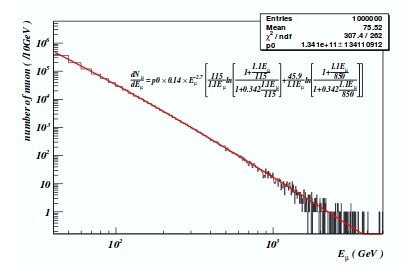
\includegraphics[]{GeisserMuon.png}
 Extra\'ido de \citep{GUAN}
\caption{Distribuci\'on de la energ\'ia de muones generada con n\'umeros aleatorios basado en la f\'ormula de Geisser}
\end{center}
\end{figure}

\subsection{CORSIKA}
Para realizar simulaciones de cómo se vería una cascada de área extensa se utiliza el programa CORSIKA. Éste simula las distintas interacciones de las distintas partículas que se van generando a partir de una primera partícula de alta energía (partícula primaria) para así construir la cascada. Éste fue creado por el Instituto de Física Nuclear de Karlsruhe (IKP) y es gratuito. Debido a la cantidad de procesos que ocurren en una simulación se necesitan supercomputadoras para realizar las simulaciones. \citep{HECK}

El modelo de Heitler es un modelo simplificado que predice el comportamiento del canal electromagnético de la cascada. Los dos mecanismos de interacción que describe son el de frenado (bremsstrahlung) y de pares: el primero es un electrón que al encontrarse con un átomo de la atmósfera desprende un electrón de menor energía y una partícula gamma, el segundo es la generación de un electrón y positrón cuando una partícula gamma se encuentra un átomo en la atmósfera. Estas interacciones cesan cuando la energía perdida por ionización del electrón es igual a su energía en reposo (otros criterios existen para para detener el proceso dentro de una simulación). \citep{SUAREZ}

Para las interacciones hadrónicas de alta energía se utilizan los modelos VENUS, QGSJET, DPMJET y SIBYLL. Para las hadrónicas de baja energía utiliza GHEISHA. Por último las electrónicas las simula con EGS4 y NKG. CORSIKA necesita que se le ingresen los siguientes datos: datos de la atmósfera en dónde se realizará la simulación, el sistema coordenado a utilizar, el campo geomagnético del lugar a simular y el sistema de unidades que se utilizará. \citep{HECK}

\section{Radiaci\'on de Vavilov-Cerenkov}
La radiaci\'on Cherenkov presenta una diferenciaci\'on marcada en relaci\'on a la luminiscencia. Esto se debe a que tanto la polarizaci\'on de las mol\'eculas, la intensidad y tiempo de excitaci\'on no son alterables.  La luz emitida en este fen\'omeno presenta una asimetr\'ia pronunciada, la cual se debe al movimiento de una part\'icula cargada a una velocidad de fase mayor a la de la luz en el medio. En donde, cada punto que es tocado por la part\'icula cargada una excitaci\'on electromagn\'etica es generada, propag\'andose en la forma -de una onda retardada desde estos puntos.  \citep{CHERENKOV}

\section{Vida media del mu\'on}

\section{Detectores Cherenkov en agua (WCD)}

\section{Geant4}

El modelo f\'isico que se utiliza para WCD es el de procesos de fotones \'opticos, bajo el modelo UNIFIED. Este modelo integra las principales caracter\'isticas de modelos \'opticos geom\'etricos y f\'isicos para reflexi\'on en superficies en diferentes longitudes de onda y aspereza.

Geant4 incluye la radiaci\'on Cherenkov como un proceso f\'isico que puede implementarse desde los archivos de procesos f\'isicos. Calcula las secciones eficaces a partir de la descripci\'on molecular del material refractor. 

%%%%%%%%%%%%%%%%Cap\'itulo nuevo

\Chapter{Antecedentes}

\section{Latin American Giant Observatory}
\subsection{Sitios de LAGO}
LAGO (Latin American Giant Observatory, por sus siglas en ingl\'es) es un proyecto internacional con m\'as de ochenta cient\'ificos de ocho pa\'ises latinoamericanos que empez\'o en 2005. Est\'a orientado principalmente a la investigaci\'on b\'asica de tres ramas de la astrof\'isica de part\'iculas: el universo en condiciones extremas, clima interplanetario y radiaci\'on atmosf\'erica a nivel del suelo. La red de detectores de LAGO consiste en un peque\~nos tanques de agua a nivel de tierra sobre diferentes localidades y latitudes a lo largo del continente latinoamericano, abarcando desde M\'exico hasta el cono sur de Am\'erica. El proyecto LAGO se ha dividi\'o en dos estudios objetivos dependiendo de la altitud del detector. Los detectores en altitudes superiores de 4,500m sobre el nivel del mar permiten detectar GRB con mayor sensibilidad; y los detectores de altitudes menores son utilizados para estudios f\'isicos del sol (Forbush Decreases). \citep{ASOREY2015}

\begin{figure}[ht] %opción h - here pone la imagen aquí en esta posición del documento
\begin{center}
 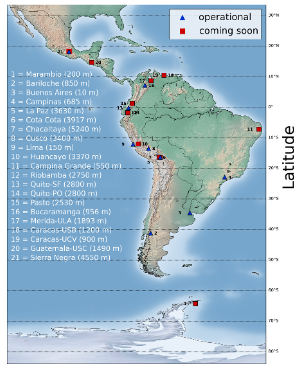
\includegraphics[width = 0.8\linewidth]{ASOREY2015.png}
 
 Extra\'ido de \citep{ASOREY2015}
\caption{Distribuci\'on geogr\'afica de los detectores de LAGO operacionales (tri\'angulos azules), y los que comenzar\'an a funcionar entre 2016 y 2017 (cuadrados rojos), y a la izquierda el umbral de rigidez vertical (vertical rigidity cutoff) del campo geomagn\'etico para cada estaci\'on.}
\end{center}
\end{figure}

Este proyecto tiene como objetivo observar Gamma Ray Bursts (GRB) (destellos de rayos gamma) utilizando detectores de agua Cherenkov (WCD). Los WCD de LAGO pueden ser utilizados para medir el flujo de rayos c\'osmicos en la tierra ya que su modulaci\'on es una medici\'on directa de la actividad solar. Por \'ultimo, los detectores instalados en universidades sirven para ense\~nar a estudiantes sobre f\'isica de part\'iculas y astropart\'iculas. Existen ya varios observatorios de LAGO en operaci\'on. Uno est\'a el de Sierra Negra, M\'exico, a 4550 metros sobre el nivel del mar. Tiene funcionando tres tanques de 4 metros cuadrados de superficie y dos de un metro cuadrado. Otro est\'a en Chacaltaya, Bolivia, a 5250 metros sobre el nivel del mar, el detector a mayor altitud de la estructura LAGO. Tiene tres tanques en operaci\'on, dos de 4 metro cuadrado y uno de 1 metro cuadrado. El otro est\'a en Marcapomacocha, Per\'u, a 4450 metros sobre el nivel del mar, con un tanque de dos metros cuadrados en operaci\'on desde el 2010. En Guatemala, ya dio inicio el proyecto en la Universidad San Carlos de Guatemala, pero a\'un no est\'a en operaci\'on. \citep{VILLASENOR}

\subsection{Calibraci\'on de datos en LAGO}

Las referencias \citep{ALLISON} y \citep{ALARCON} describen c\'omo utilizar informaci\'on de eventos de muones secundarios en el tanque para calibrar los datos a partir de eventos de muones verticales equivalentes (VEM). El VEM es la medida de la se\~nal m\'axima obtenida de la distribuci\'on de carga de muones que cruzan verticalmente. Esta medida se puede obtener de los histogramas de carga integrada obtenidos de los programas cal.cc y sol.cc aplicados a datos obtenidos de ACQUA. El valor de VEM es el valor de carga integrada (medida en ADCq) que corresponde al segundo m\'aximo de figura obtenida. Dos m\'etodos para obtener este valor es a trav\'es de regresi\'on cuadr\'atica o diferenciaci\'on finita. Este valor se obtendr\'a tambi\'en con la simulaci\'on, de manera directa.

En los histogramas de carga arrojados por sol.cc y cal.cc, se revela adem\'as el tipo de part\'icula de la lluvia que inciden en el detector. En \citep{ASOREY} estos histogramas se utilizaron para dividir las se\~nales en cuatro bandas: la electromagn\'etica (para valores de ADCq menores al valor de transici\'on), la mu\'onica (que incluye el valor de VEM), las part\'iculas de mini-lluvias (arriba del l\'imite del mu\'on de m\'axima trayectoria), y una cuarta banda que re\'une muones desde el VEM hasta el resto de part\'iculas sobre este valor. \citep{Yunior}

Para el monitore, los datos del WCD deben deben de corregirse por la anticorrelaci\'on entre presi\'on atmosf\'erica y conteo de part\'iculas secundarias para el monitoreo de clima solar. Esta correcci\'on es de tipo multiplicativa ya que la variaci\'on de la presi\'on atmosf\'erica es local. \citep{Yunior} \citep{ASOREY}

\section{Observatorio Pierre Auger}

Por otro lado, la instalaci\'on m\'as grande de detectores de agua de radiaci\'on Cherenkov es Pierre Auger, en Argentina. Consiste en 1660 tanques de agua dispuestos en una regi\'on triangular de 3000 kil\'ometros cuadrados, espaciados a 1500 metros. El arreglo en Pierre Auger tiene un \'area total de $16000m^{2}$ y funciona a $10^8$ conteos por minuto. Algunas especificaciones del modelo Scaler en Pierre Auger: Muestreo de 40MHz por seis 10-bit flash analog-to-digital converter (FADC), enlace de radio al CDAS (central data acquisition system), sistema GPS para sincronizar los 1660 tanques. Un \'area total de 16000m2 y mil millones de conteos por minuto. La respuesta del detector est\'a hecha de un conjunto de simulaciones de showers de baja energ\'ia usando CORSIKA 6.980 modelo QGSJET-II para hadrones alta energ\'ia y GHEISHA para bajas. El flujo de part\'iculas primarias a 100 km se simula como una ley de poder, cuyo exponente se obtuvo de mediciones de espectro de energ\'ias de la part\'icula primaria. \citep{VILLASENOR}

\section{Uso de Geant4 en LAGO y otros experimentos}

Para realizar las simulaciones de GEANT4 se siguieron las gu\'ias de desarrollador de aplicaci\'on y se tomar\'an de referencias otros art\'iculos con simulaciones parecidas, \citep{NIELSEN}, \citep{CHEN}, \citep{CALDERON}.

%%%%%%%%%%%%%%%%Cap\'itulo nuevo

\Chapter{Metodolog\'ia}

\section{Instalaci\'on del WCD}

\section{Calibraci\'on por histograma de datos del WCD}

\section{Vida media del mu\'on con datos del WCD}

\section{Geant4}
\subsection{Geometr\'ia}
\subsubsection{Objetos y colocaci\'on}

Los objetos de la construcci\'on del detector relevantes para la simulaci\'on son los objetos con los que interact\'uan los fot\'ones \'opticos y los secundarios incidentes dentro del tanque. Estos objetos son el recubrimiento de Tyvek, que se toma como un capa cil\'indrica, el agua dentro del Tyvek, la superficie de vidrio borosilicato del fotomultplicador y el fotoc\'atodo de aluminio, ambos tomados como semiesferas. Geant4 permite organizar objetos seg\'un jerarqu\'ias: el cuadro 6.1 describe la forma, dimensiones y colocaci\'on de los objetos y sus jerarqu\'ias bajo los respectivos vol\'umenes madre. Las dimensiones del Tyvek y de las semiesferas que conforman la parte del fotomultiplicador en contacto con el agua fueron medidas directamente del tanque del experimento. Esta geometr\'ia se ve claramente en la figura 6.1.

\begin{table}[ht]
\caption{ Descripci\'on de los objetos en la simulaci\'on y sus jerarquías lógicas}
\centering
\begin{tabular}{l c c c c }
\hline
Nombre & \specialcell{Volumen madre\\(posici\'on)} & Material & Tipo & Dimensiones  \\

 \hline
\hline
World & ninguno & Aire & G4Box & 1 metro por lado\\
Tyvek & \specialcell{World\\(0,0,0)} & Tyvek & G4Cons & \specialcell{Radio interno a = 0m\\Radio interno b = 0m\\ Radio externo a = 40.1m\\Radio externo b = 40.1m\\Altura = 57.1cm\\\'Angulo m\'inimo = $0^o$\\\'Angulo m\'aximo = $360^o$}\\
Agua & \specialcell{Tyvek\\(0,0,0)} & Agua & G4Cons & \specialcell{Radio interno a = 0m\\Radio interno b = 0m\\ Radio externo a = 40.0m\\Radio externo b = 40.0m\\Altura = 57.0cm\\\'Angulo m\'inimo = $0^o$\\\'Angulo m\'aximo = $360^o$}\\
Vidrio PMT & \specialcell{Agua\\(0,0,57cm)} & Borosilicato & G4Sphere & \specialcell{Radio interno = 0.0m\\Radio externo = 11.4cm\\\'Angulo $\phi$ m\'inimo = $0^o$\\\'Angulo $\phi$ que abarca = $360^o$\\\'Angulo $\theta$ m\'inimo = $0^o$\\\'Angulo $\theta$ que abarca = $360^o$}\\
Fotocátodo PMT & \specialcell{Vidrio PMT\\(0,0,0)} & Aluminio & G4Sphere & \specialcell{Radio interno = 0.0m\\Radio externo = 11.1cm\\\'Angulo $\phi$ m\'inimo = $0^o$\\\'Angulo $\phi$ que abarca = $360^o$\\\'Angulo $\theta$ m\'inimo = $0^o$\\\'Angulo $\theta$ que abarca = $360^o$}\\
\hline
\end{tabular}
\end{table}

\begin{figure}[ht] %opción h - here pone la imagen aquí en esta posición del documento
\begin{center}
 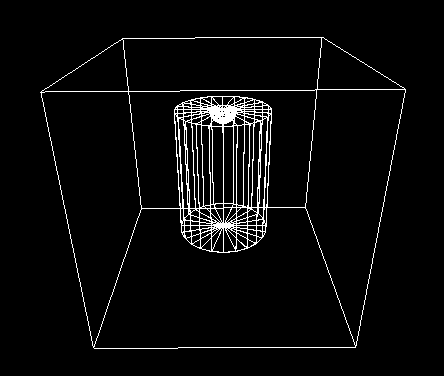
\includegraphics[width = 0.8\linewidth]{GeometriaG4.png}
 
(Fuente propia)
\caption{Esquema de la geometr\'ia general del detector en la simulaci\'on Geant4, mostrando el recubrimiento Tyvek en forma cil\'indrica y las superficies de vidrio y fotoc\'atodo del fotomultiplicador}
\end{center}
\end{figure}

\subsubsection{Materiales}
\subsubsection{Superficies}

\subsection{Detecci\'on}
\subsubsection{Asignaci\'on de superficies sensibles}
\subsubsection{Criterio de detecci\'on}

\subsection{Generaci\'on de evento}
\subsubsection{Procesos f\'isicos}
\subsubsection{Posici\'on y direcci\'on}
\subsubsection{Espectro de energ\'ia de muones}

\subsection{Datos de salida}
\subsubsection{Forma del pulso}
\subsubsection{Histograma de carga para muones}
%%%%%%%%%%%%%%%%Cap\'itulo nuevo

\Chapter{Resultados}

%%%%%%%%%%%%%%%%Cap\'itulo nuevo

\Chapter{Discusi\'on}

% % % % % % % % % % % % % % % % % % % % % % %                       Secci\'on de bibliograf\'ia

\Biblio
\begin{thebibliography}{9}
\Bibliotoc
\bibitem[Alarc\'on, M. et al (1999)]{ALARCON} Alarc\'on, M. et al. 1999. \textit{Calibration and monitoring of water Cherenkov detectors with stopping and crossing muons}. Nuclear Instruments and Methods in Physics. Research A 420: 39-47. Disponible en: http://www.ung.si/public/pao/bibl/nim\_420\_ma.pdf [con acceso el 16 de noviembre del 2015]

\bibitem[Allison, P. et al. (2005)]{ALLISON} Allison, P. et al. 2005. \textit{Observing muon decays in water Cherenkov detectors at Pierre Auger Observatory}. 29th International Cosmic Ray Conference Pune 00, 101-104. Disponible en: http://arxiv.org/pdf/astro-ph/0509238.pdf [tomado el 16 de noviembre del 2015]


\bibitem[Asorey, H. (2012)]{ASOREY} Asorey, H. 2012. \textit{Los detectores Cherenkov del observatorio Pierre Auger y su aplicaci\'on al estudio de fondos de radiaci\'on}. Tesis Universidad Nacional de Cuyo. 286 p\'aginas.

\bibitem[Asorey, H. y S. Dasso (2015)]{ASOREY2015} Asorey, H. y S. Dasso. 2015. \textit{LAGO: the Latin American Giant Observatory}. The 34th International Cosmic Ray Conference. The Hague, Pa\'ses Bajos.

\bibitem[Calderon, R., H. Asorey y L. N\'u\~nez (2005)]{CALDERON} Calderon, R, H. Asorey y L. N\'u\~nez \textit{Geant4 based simulation of the Water Cherenkov Detectors of the LAGO project}. Disponible en: http://arxiv.org/pdf/1503.07270.pdf [consultado el 4 de julio 2016]

\bibitem[Chen, M. et al. (2006)]{CHEN} Chen, M. et al. 2006. \textit{A study of the water Cherenkov calorimeter}. Preimpresión presentada a Eliver Science. Disponible en: http://arxiv.org/pdf/physics/0602169.pdf [consultado el 15 de marzo del 2016]

\bibitem[Cherenkov, P. (1958)]{CHERENKOV} Cherenkov, P. 1958. \textit{Radiation of particles moving at a velocity exceeding that of light, and some of the possibilities for their use in experimental physics}. Nobel Lecture. P. 15.

\bibitem[Dasso, S. y H. Assorey (2012)]{DASSO} Dasso, S. y H. Assorey. 2012. {\title The Scaler Mode in Pierre Auger Observatory to study heliospheric modulations of cosmic rays}. arXiv:1204.6196


\bibitem[Geant4 User's Guide (2015)]{GEANT4} Geant4. 2015. \textit{Geant4 User's Guide – For Application Developers -}. Disponible en:\\ http://geant4.web.cern.ch/geant4/G4UsersDocuments/UsersGuides/ForApplicationDeveloper\\/html/index.html [consultado el 15 de mayo del 2016]

\bibitem[Guan et al. (2006)]{GUAN} Guan, M. et al. 2006.  \textit{Muon Simulation at the Daya Bay site}. Disponible en: \\http://www.osti.gov/scitech/servlets/purl/1006397 [con acceso el 17 de octubre del 2016]

\bibitem[Heck, D. et al (1998)]{HECK} Heck, D. 1998. \textit{CORSIKA: A Monte Carlo code to simulate Extensive Air Showers}. Disponible en: https://web.ikp.kit.edu/corsika/physics\_description/corsika\_phys.pdf [con acceso el 18 de marzo del 2016]

\bibitem[Lukens, J., B. Reid y A. Tuggle (2010)]{LUKENS} Lukens, J., B. Reid y A. Tuggle.  2010. \textit{Experiment in muon Decay}. Universidad de Alabama.

\bibitem[Nielsen, C. (2010)]{NIELSEN} Nielsen, C.  2010. \textit{Calibration Through Simulation of a Low-Energy Cherenkov Detector}. Tesis University of California, Santa Barbara. Disponible en: http://www.physics.ucsb.edu/sites\\/secure.lsit.ucsb.edu.phys.d7/files/sitefiles/education/ Nielsen.pdf [con acceso el 2 de junio del 2016]

\bibitem[Suarez (2014)]{SUAREZ} Suarez, M. 2014. \textit{Seminario Cascadas A\'ereas Extensas (EAS) para la colaboraci\'on LAGO, Sesi\'on 2}. Disponible en: https://www.youtube.com/watch?v=AP9i5pdbJNc [con acceso el 2 de septiembre del 2015]

\bibitem[Villase\~nor et al (2011)]{VILLASENOR} Villase\~nor, L. y et al. 2011. \textit{Search for Gamma Ray Bursts and Forbush Decreases in the LAGO Observatory}. International Cosmic Ray Conference, Beijing. $(10)$: 314.

% \bibitem[Como aparece al citar]{referencia} Datos Bibliogr\'aficos

\end{thebibliography}



 % % % % % % % % % % % % % % % % % % % % % %                                   Ap\'endices

\Chapter{Anexos}

\end{document}

